\chapter{Nosso dinheiro}
\markboth{Módulo 6}{}

\section*{Habilidades do SAEB}

\begin{itemize}
\item Relacionar valores de moedas e/ou cédulas do sistema monetário
brasileiro, com base nas imagens desses objetos.

\item Resolver problemas que envolvam moedas e/ou cédulas do sistema
monetário brasileiro.
\end{itemize}

\subsection{Habilidade da BNCC}

\begin{itemize}
  \item 
 EF03MA24.
\end{itemize}

\conteudo{
\begin{center}
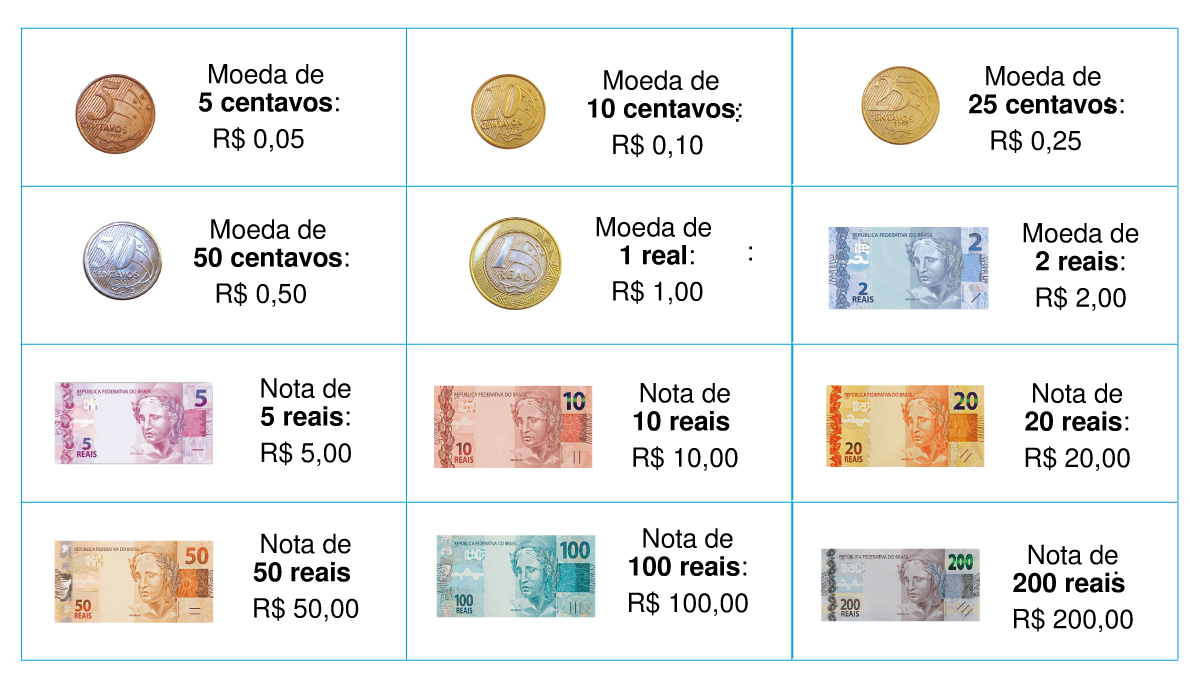
\includegraphics[width=\textwidth]{./media/image64.png}
\end{center}}

\pagebreak

\section*{Atividades}

\begin{comment}
\num{1} Complete o quadro, relacionando o valor das cédulas e moedas do
sistema monetário brasileiro com seu valor e com como se lê esse valor.

\begin{longtable}[]{@{}lll@{}}
\toprule
\hline
\vspace{1em}
\textbf{Cédula ou moeda} & \textbf{Valor} & \textbf{Como se lê}\tabularnewline
\hline
\midrule
\endhead
\vspace{1em}
Nota de 200 reais & \rosa{R\$ 200,00} & Duzentos reais\tabularnewline
\hline
\vspace{1em}
Nota de 100 reais & \rosa{R\$ 100,00} & \rosa{Cem reais}\tabularnewline
\hline
\vspace{1em}
Nota de 50 reais & \rosa{R\$ 50,00} & \rosa{Cinquenta reais}\tabularnewline
\hline
\vspace{1em}
Nota de 20 reais & R\$ 20,00 & \rosa{Vinte reais}\tabularnewline
\hline
\vspace{1em}
Nota de 10 reais & \rosa{R\$ 10,00} & \rosa{Dez reais}\tabularnewline
\hline
\vspace{1em}
Nota de 5 reais & \rosa{R\$ 5,00} & Cinco reais\tabularnewline
\hline
\vspace{1em}
Nota de 2 reais & \rosa{R\$ 2,00} & \rosa{Dois reais}\tabularnewline
\hline
\vspace{1em}
Moeda de 1 real & \rosa{R\$ 1,00} & \rosa{Um real}\tabularnewline
\hline
\vspace{1em}
Moeda de 0,50 centavos & R\$ 0,50 & \rosa{Cinquenta
centavos}\tabularnewline
\hline
\vspace{1em}
Moeda de 0,25 centavos & \rosa{R\$ 0,25} & \rosa{Vinte e cinco
centavos}\tabularnewline
\hline
\vspace{1em}
Moeda de 0,10 centavos & \rosa{R\$ 0,10} & \rosa{Dez centavos}\tabularnewline
\hline
\vspace{1em}
Moeda de 0,05 centavos & \rosa{R\$0,05} & Cinco centavos\tabularnewline
\hline
\bottomrule
\end{longtable}
\end{comment}

\num{1} André foi ao banco efetuar um saque (retirada de dinheiro de sua conta
bancária) e, ao pegar o valor pretendido, recebeu as seguintes cédulas e moedas:

\begin{figure}[htpb!]
\centering
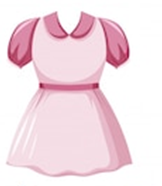
\includegraphics[width=\textwidth]{./media/image65.png}
\end{figure}

Qual o valor que André retirou de sua conta bancária?
\reduline{1 x 50 + 4 x 20 + 1 x 10 + 3 x 5 + 2 x 2 + 2 x 1 + 5 x 0,50 = 50 + 80 +
10 + 15 + 4 + 2 + 2,5 = R\$ 163,50.\hfill}
\linhas{4}

\pagebreak
\num{2} A mãe de Leonardo foi ao supermercado. Ela comprou um pacote de açúcar mascavo, três unidades de suco, um pacote de arroz integral, um queijo, uma manteiga e um pacote de café.

Observando o preço de cada produto e a quantidade que ela adquiriu, qual é o valor que ela gastou? 

\begin{figure}[htpb!]
\centering

\includegraphics[width=.8\textwidth]{./media/image66.png}
\end{figure}

\reduline{Açúcar mascavo: 1 x R\$: 5,00; suco: 3 x R\$ 3 = R\$ 9,00; arroz integral: 1 x R\$ 10,00; queijo: 1 x R\$ 19,00; manteiga: R\$ 15,00; café: R\$ 9,00. Valor total: 5 + 9 + 10 + 19 + 15 + 9 = R\$ 67,00.}

\num{3} Uma grande rede de lojas realizou uma promoção de vendas após o Natal.
Veja os produtos que estavam em promoção e seus respectivos preços.

\begin{figure}[htpb!]
\centering
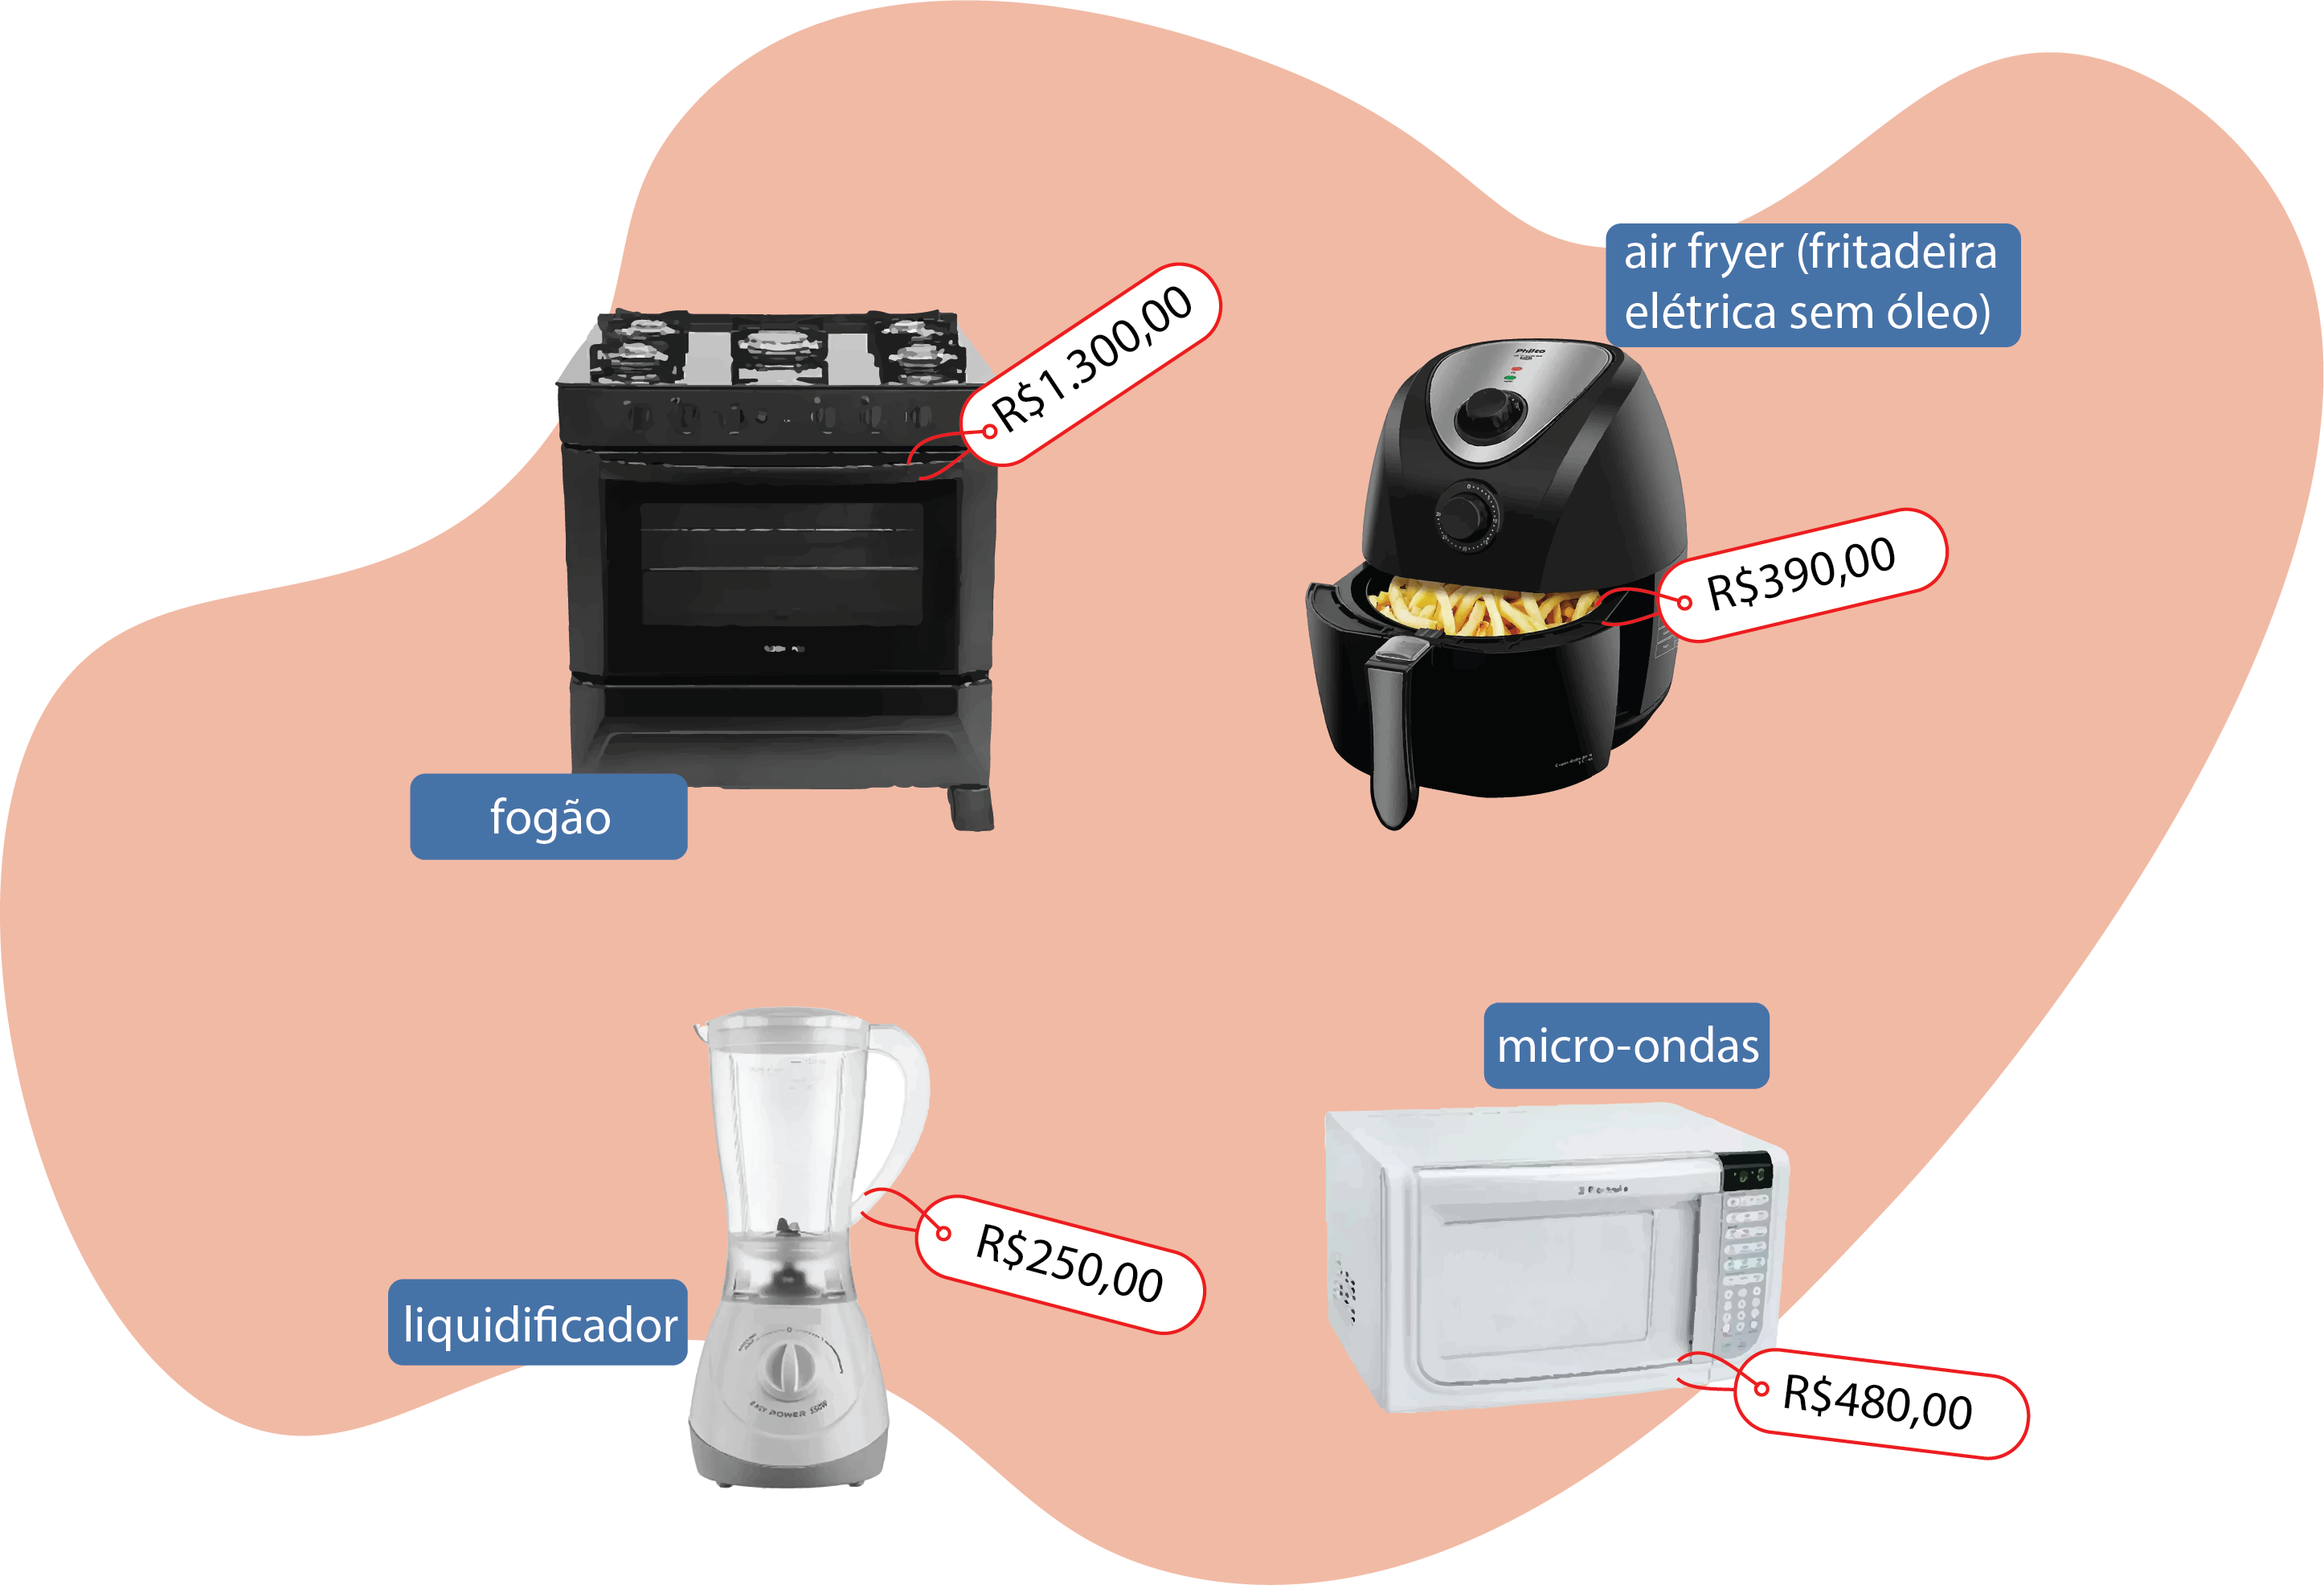
\includegraphics[width=.6\textwidth]{./media/image67.png}
\end{figure}

\pagebreak

Observavdo a figura, responda a cada item.

\begin{escolha}
\item Se uma pessoa comprar um fogão e um liquidificador, quanto irá pagar?
\reduline{1.300 + 250 = R\$ 1.550,00.\hfill}

\item Se uma pessoa conseguir um desconto de R\$ 50,00 para pagamento à
  vista na compra do microondas, qual será o valor que ela pagará?
\reduline{480 - 50 = R\$ 430,00.\hfill}
\end{escolha}

\num{4} O quadro a seguir mostra a pesquisa de preços que José está fazendo
de um jogo de videogame e um controle bluetooth.

\begin{longtable}[]{@{}lll@{}}
\toprule
\hline
\textbf{Produto} & \textbf{Loja A} & \textbf{Loja B}\tabularnewline
\hline
\midrule
\endhead
\textbf{Jogo de videogame} & R\$ 200,00 & R\$ 176,00\tabularnewline
\hline
\textbf{Controle bluetooth} & R\$ 616,00 & R\$ 654,00\tabularnewline
\hline
\hline
\textbf{Total} & \textbf{R\$} & \textbf{R\$}\tabularnewline
\bottomrule
\end{longtable}

\begin{figure}[htpb!]
\centering
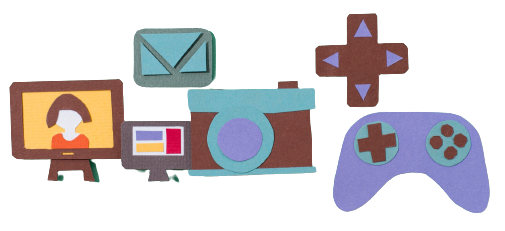
\includegraphics[width=.6\textwidth]{./media/image67a.png}
\end{figure}

\begin{escolha}
\item Se José comprar os dois itens na loja A, pagará quanto?
\reduline{200 + 616 = R\$ 816,00\hfill}

\item Se optar por comprar tuda na loja B, qual o valor que pagará?
\reduline{176 + 654 = R\$ 830,00\hfill}

\item Se ele quer pagar o menor preço possível, determine em qual loja ele
  deverá comprar cada item e calcule qual o valor que pagará.
\reduline{Ele deverá comprar o jogo na loja B por R\$ 176,00 e o controle na
  loja A por R\$ 616,00. Com isso, pagará R\$ 792,00.\hfill}
\end{escolha}

\num{5} Marta foi à papelaria comprar uma caneta de que estava precisando para
continuar seus estudos. Ela comprou uma caneta que custava 7 reais e 75
centavos. Sabendo-se que ela pagou com uma nota de 10 reais, quais
cédulas e moedas ela recebeu de troco?
\reduline{Como o enunciado indica que são cédulas e moedas, ela deve ter recebido
de troco uma nota de 2 reais e 1 moeda de 25 centavos.
%Existem outras opções que podem ser exploradas.
%Explorar com os alunos outras situações para que treinem um
%pouco esse conceito. Além disso, converse um pouco com os alunos sobre
%outras moedas que existem no mundo e qual o seu valor em relação ao real
%e vice-versa.
\hfill}

\num{6} Caíque queria economizar  dinheiro. Para isso, decidiu comprar um videogame usado
que custava R\$ 3.490,00 à vista. Ele ainda conversou com o vendedor e pediu
um desconto. O vendedor concedeu  uma redução de R\$ 350,00. Quanto ele pagou pelo videogame?
\reduline{R\$ 3.490,00 -- R\$ 350,00 = R\$ 3.140,00\hfill}
\linhas{2}

\num{7} Em muitas compras a prazo, é exigida uma entrada que é paga no ato da
compra, e o restante do valor pode ser dividido em um número combinado de
parcelas mensais. Veja o exemplo.

\begin{figure}[htpb!]
\centering
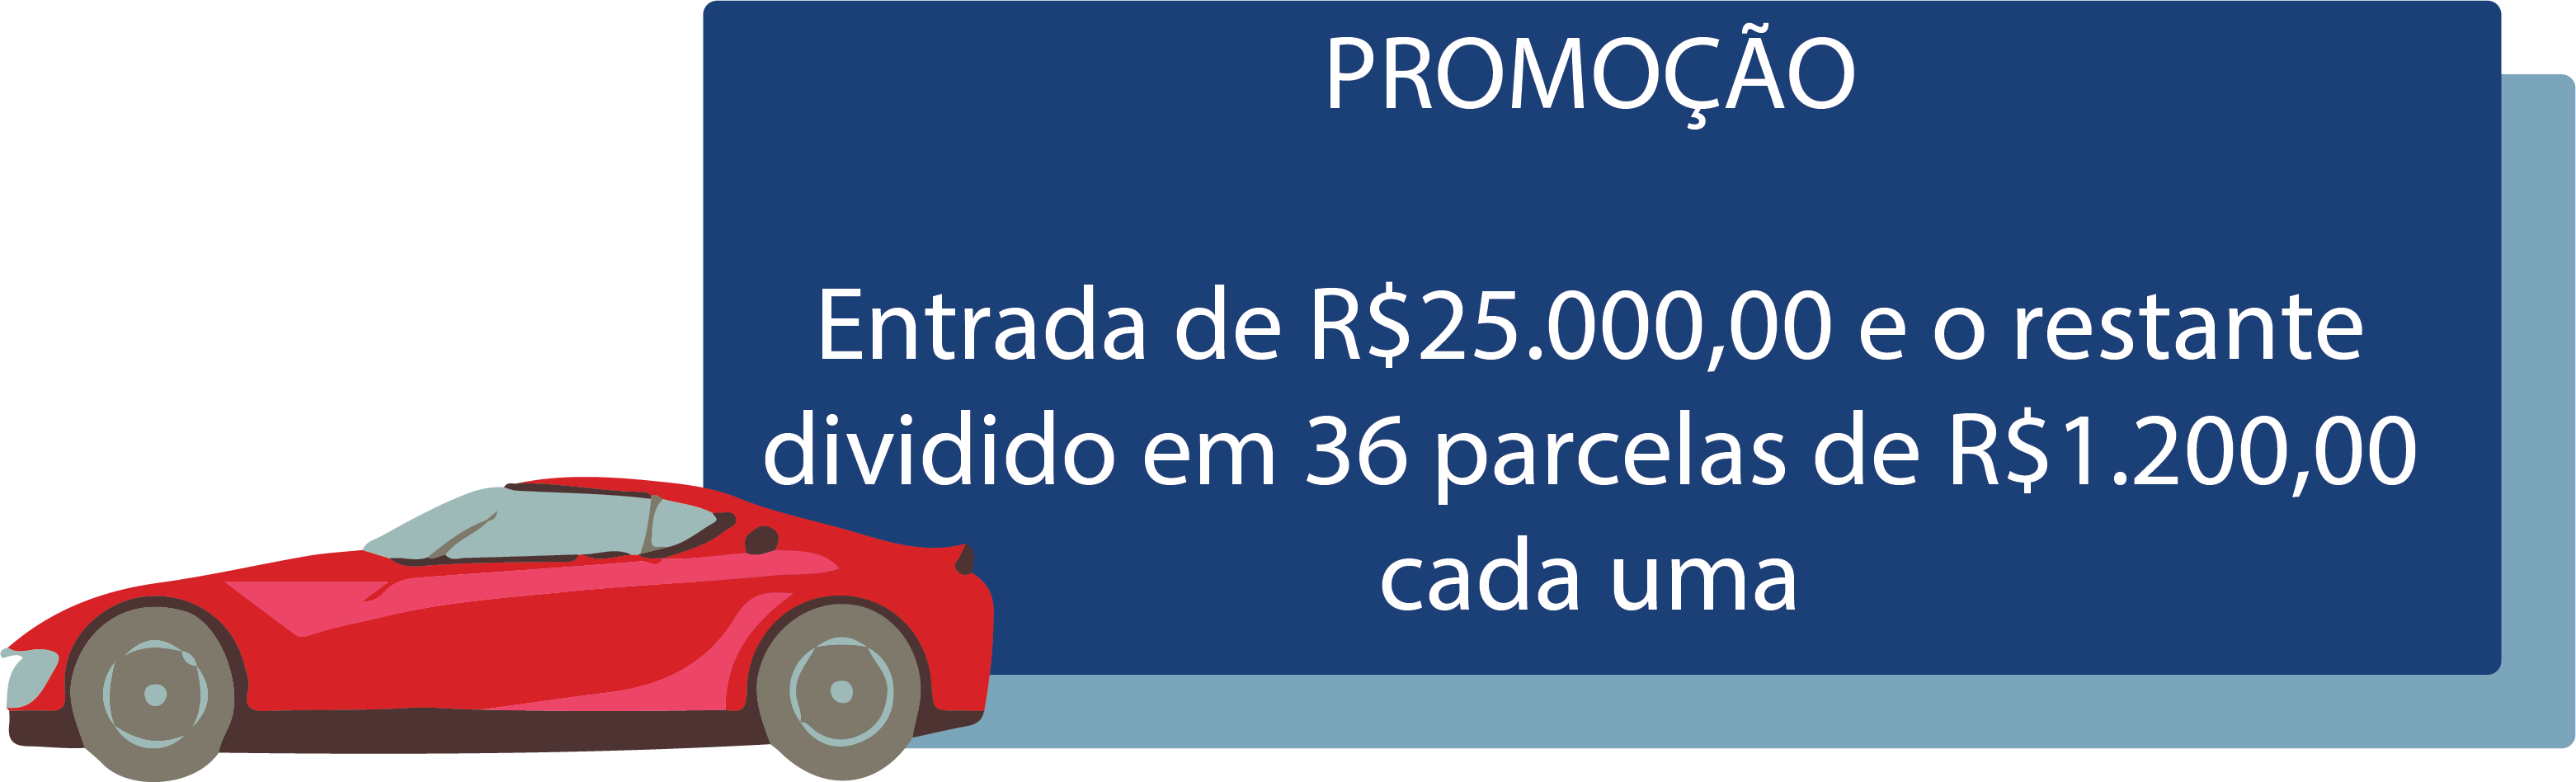
\includegraphics[width=\textwidth]{./media/image68.png}
\end{figure}

\begin{escolha}
\item Qual o valor que será dividido em 24 vezes?
\reduline{24 x 1.200 = R\$ 28.800,00\hfill}

\item Qual o valor que cada parcela terá?
\reduline{Lendo atentamente o texto, sabe-se que cada parcela será de R\$ 1.200,00\hfill}

\item Se a loja fornece um desconto à vista de R\$ 2.580,00, quem optar por
  comprar dessa forma pagará quanto pelo carro?
\reduline{25.000 + (24 x 1.200) - 2.580 = R\$ 51.220,00\hfill}
\end{escolha}

%\coment{Incentive os alunos a fazer a montagem da expressão, mesmo que encontrem outra saída de resolução. É importante não inibir outras resoluções, mas sim mostrar várias formas e, dentre elas, a montagem da expressão.}

\num{8}  Complete os quadros com as quantidades de cada nota para que se
obtenham os valores estipulados.

\begin{figure}[htpb!]
\centering
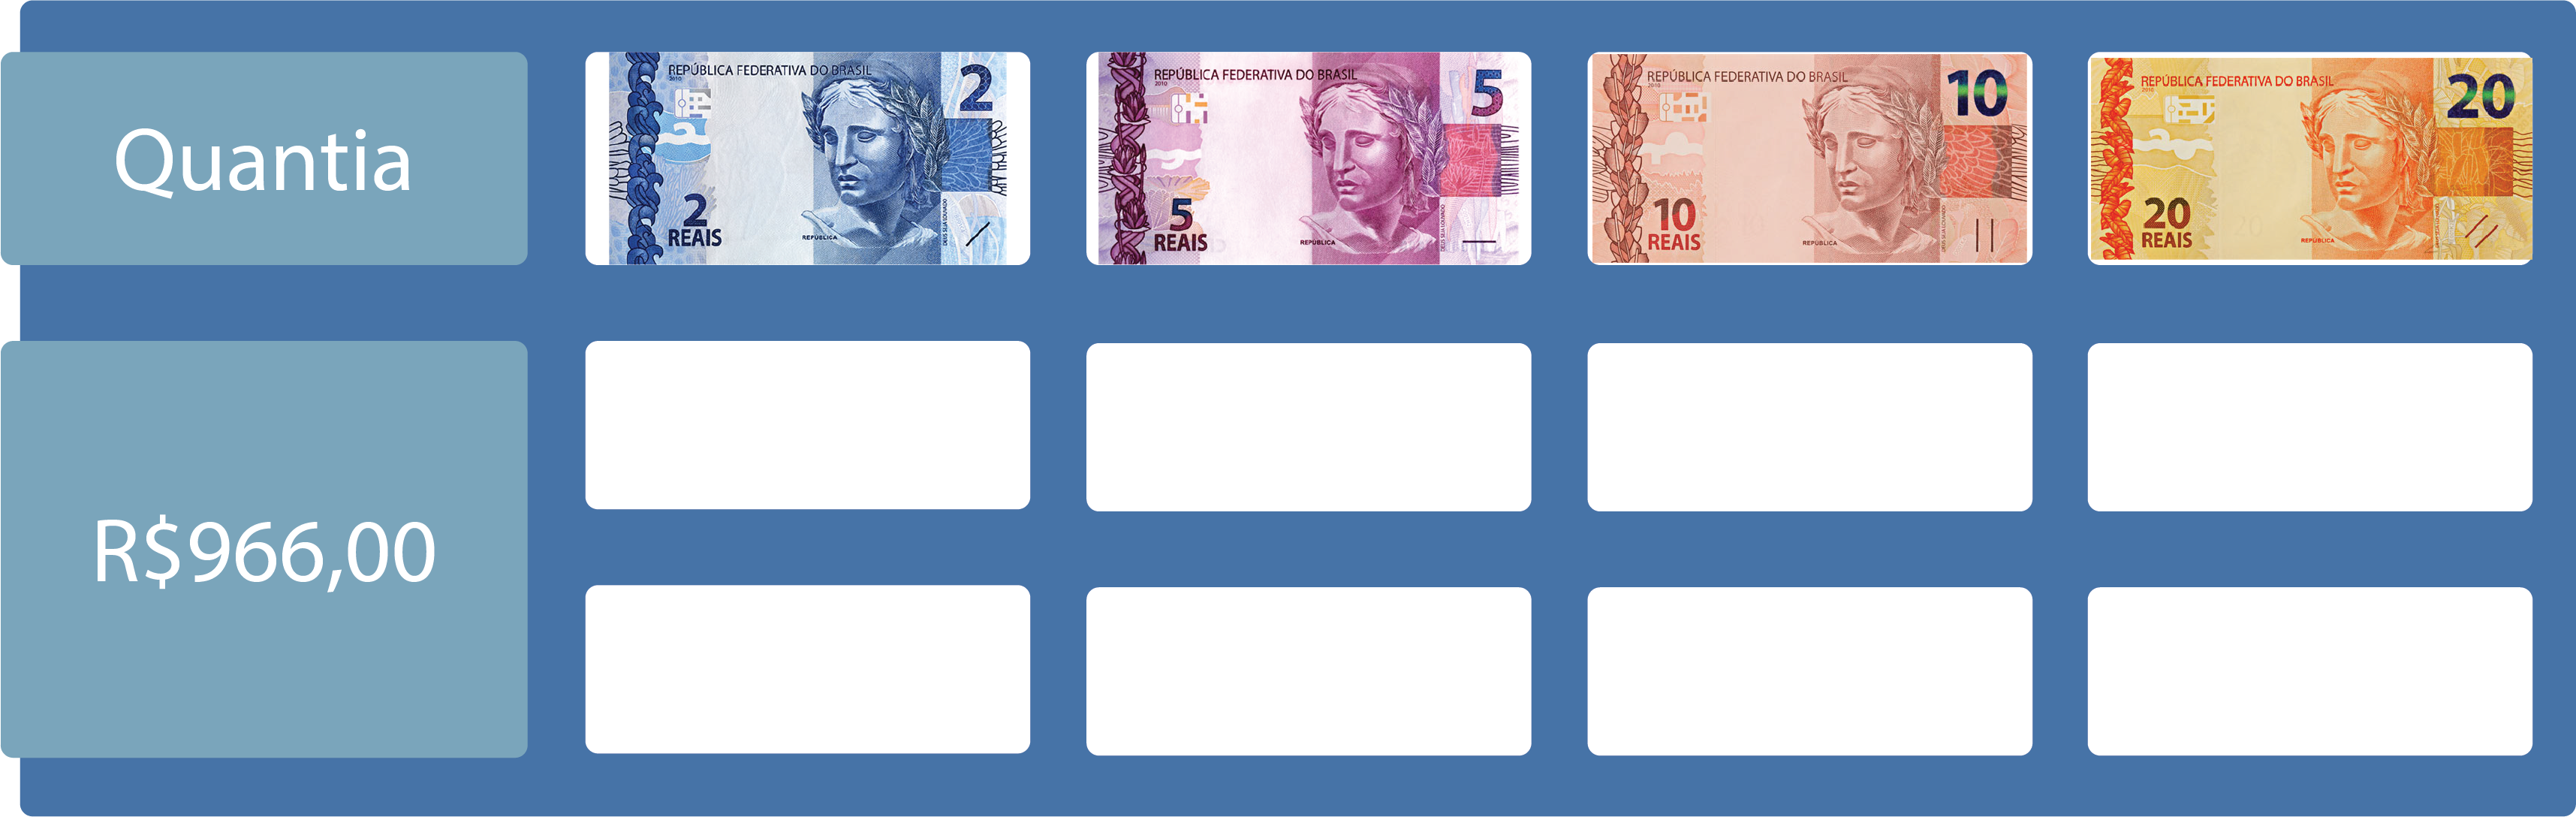
\includegraphics[width=\textwidth]{./media/image69.png}
\end{figure}

\begin{figure}[htpb!]
\centering
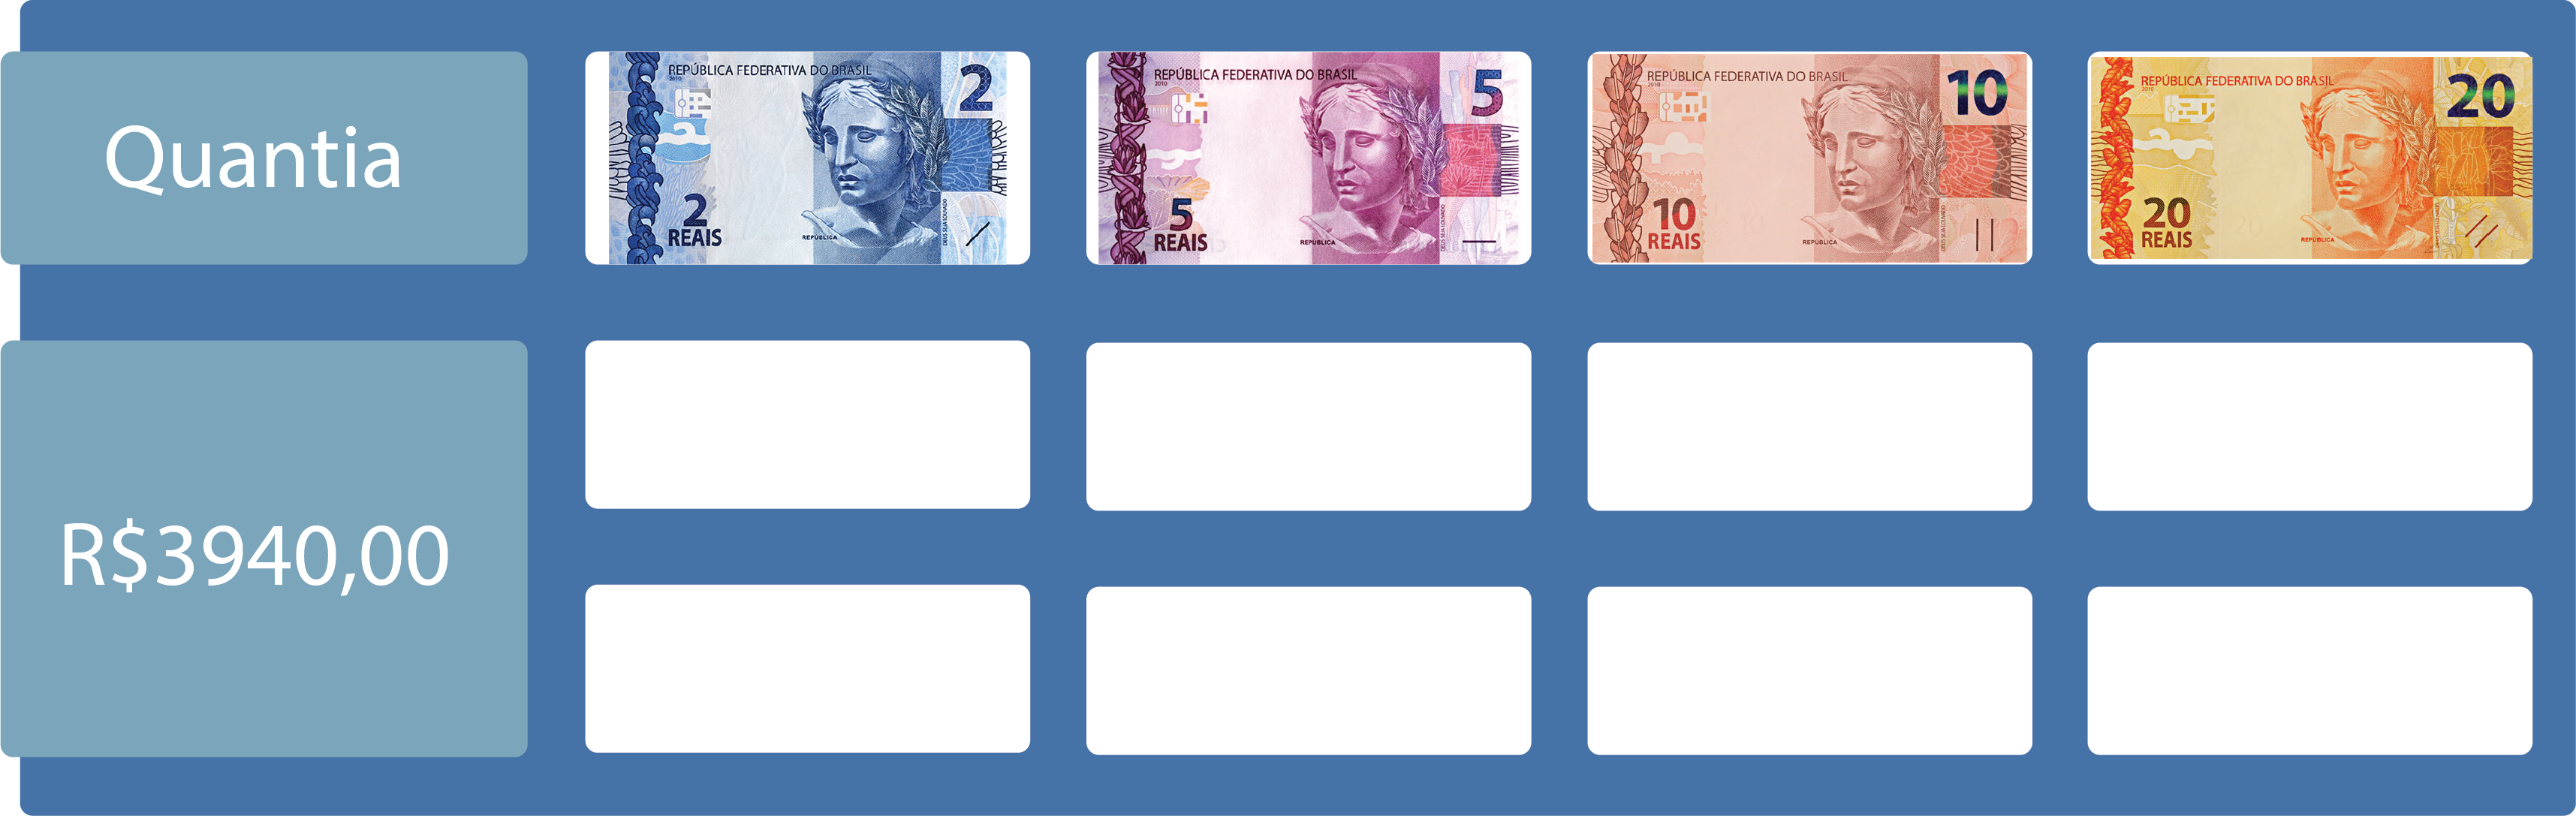
\includegraphics[width=\textwidth]{./media/image70.png}
\end{figure}

%\coment{
%Podem surgir outras combinações para a resposta. Incentive e estimule essa criatividade.
%A) Uma possibilidade para R\$ 966,00 podem ser 48 notas de 20 reais e 3
%  notas de 2 reais.
%B) Uma possibilidade para R\$ 3.940,00 podem ser 15 notas de 200 reais, 9
% notas de 100 reais e 2 notas 20 reais.}

\pagebreak
\num{9} Bianca foi a uma loja comprar um presente para sua filha e se deparou
com os seguintes objetos e seus respectivos preços:

\begin{figure}[htpb!]
\centering
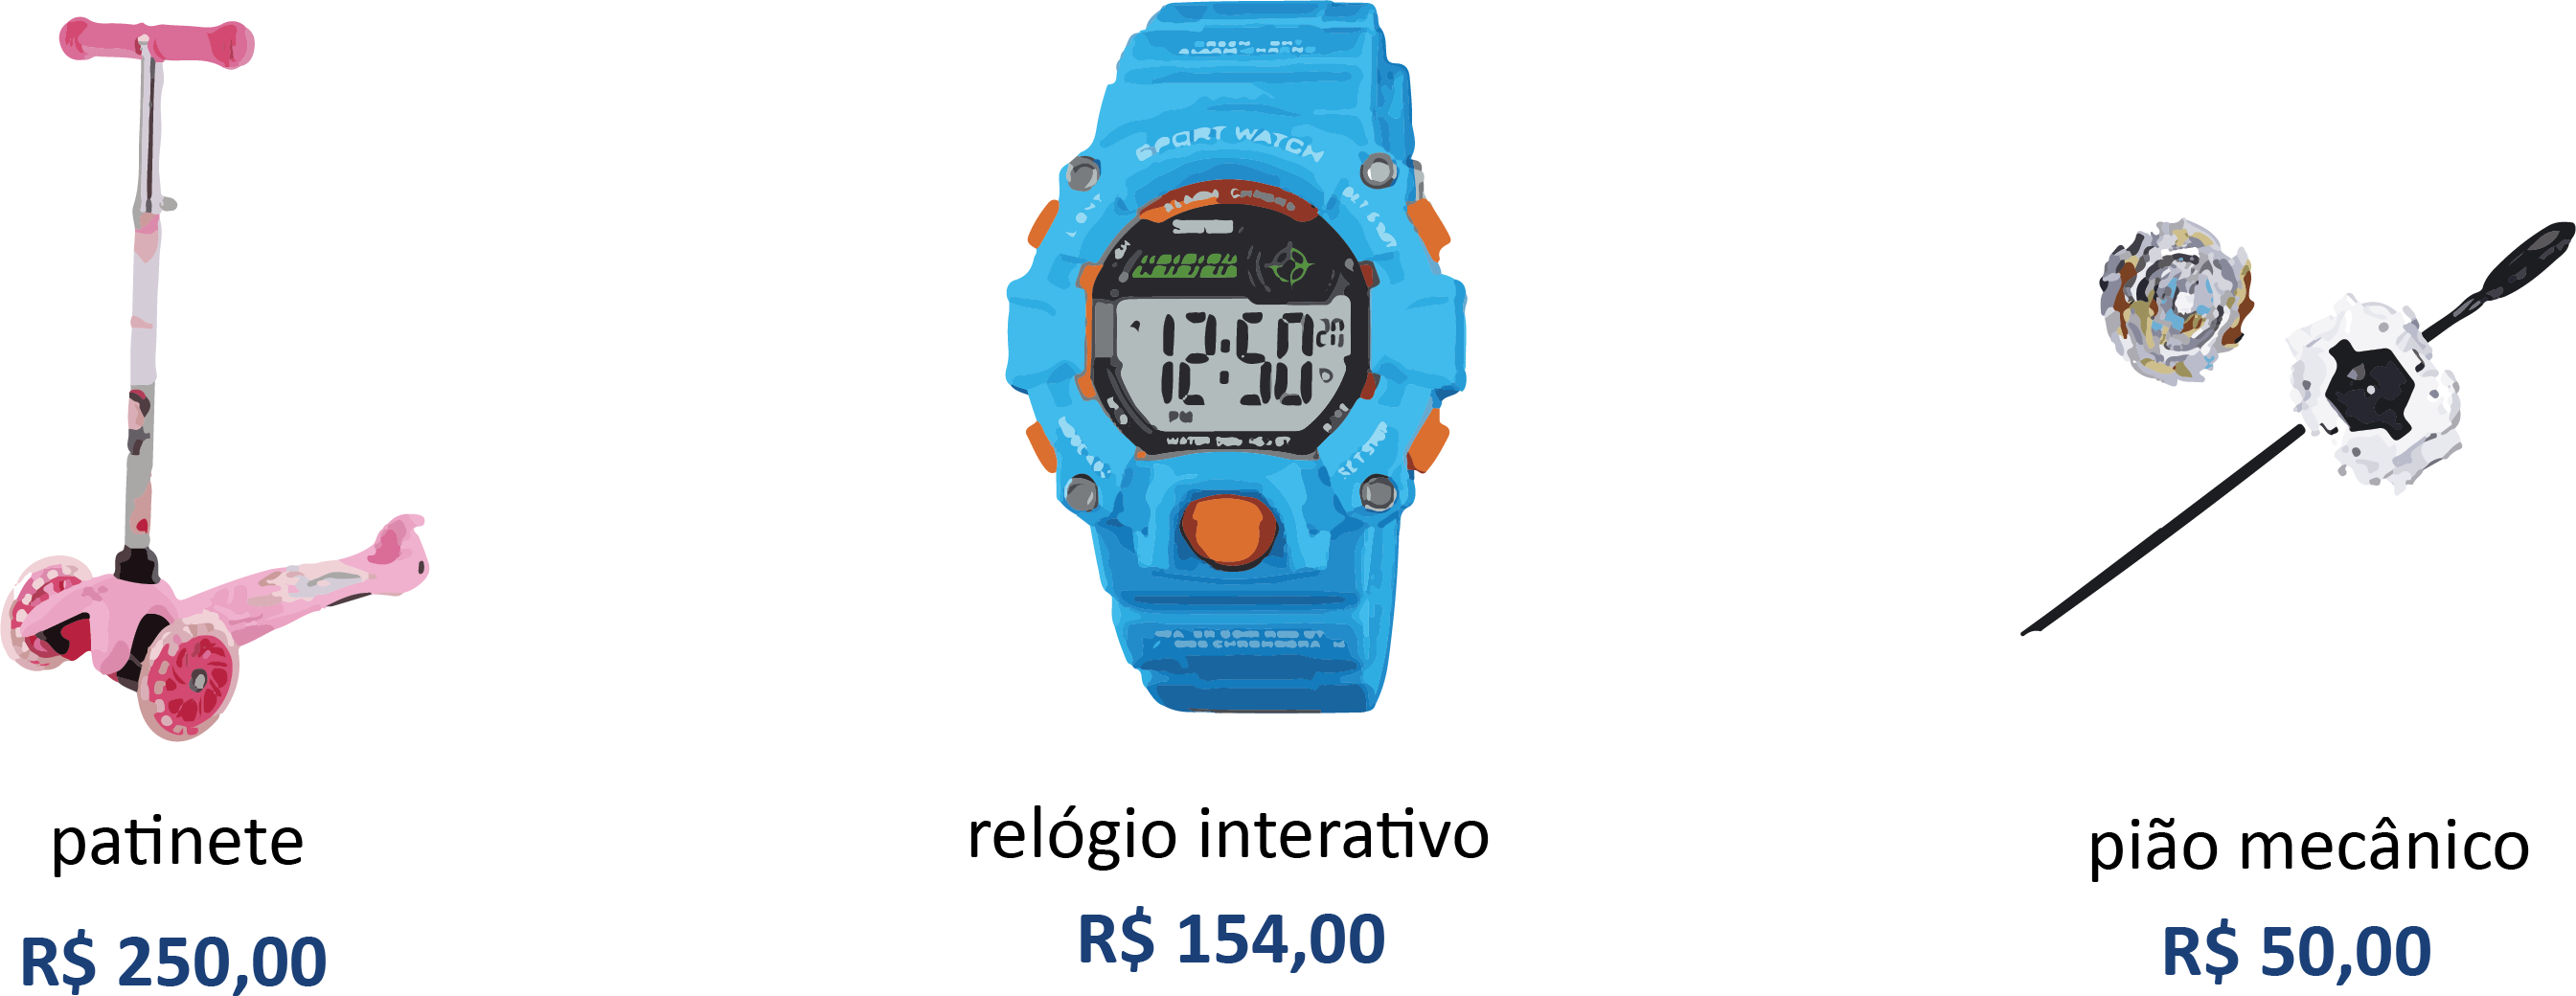
\includegraphics[width=\textwidth]{./media/image72.png}
\end{figure}

Observe atentamente a figura e, em seguida, responda a cada um dos itens.

\begin{escolha}
\item Qual dos três objetos é o mais barato?
\reduline{O mais barato é o pião mecânico, no valor de R\$ 50,00.\hfill}
\linhas{1}

\item Se Bianca resolveu comprar o patinete e o relógio, quanto ela gastou?
\reduline{250 + 154 = R\$ 404,00\hfill}
\linhas{1}
\end{escolha}

\num{10} Jonas recebe pelo seu trabalho R\$ 550,00 por semana. Na segunda-feira, usou R\$ 100,00 para pagar a conta de luz. Na terça-feira, desembolsou R\$ 50,00 reais no transporte. E, na quarta-feira, empregou R\$ 120 reais em alimentação. Quanto ele ainda dispõe para passar o restante da semana?
\reduline{550 -- 100 -- 50 -- 120 = 350 -- 270 = R\$ 280,00\hfill}

\pagebreak
\section*{Treino}

\num{1} Felipe, vendo alguns anúncios de televisores na internet, encontrou um que dizia:

\begin{figure}[htpb!]
\centering
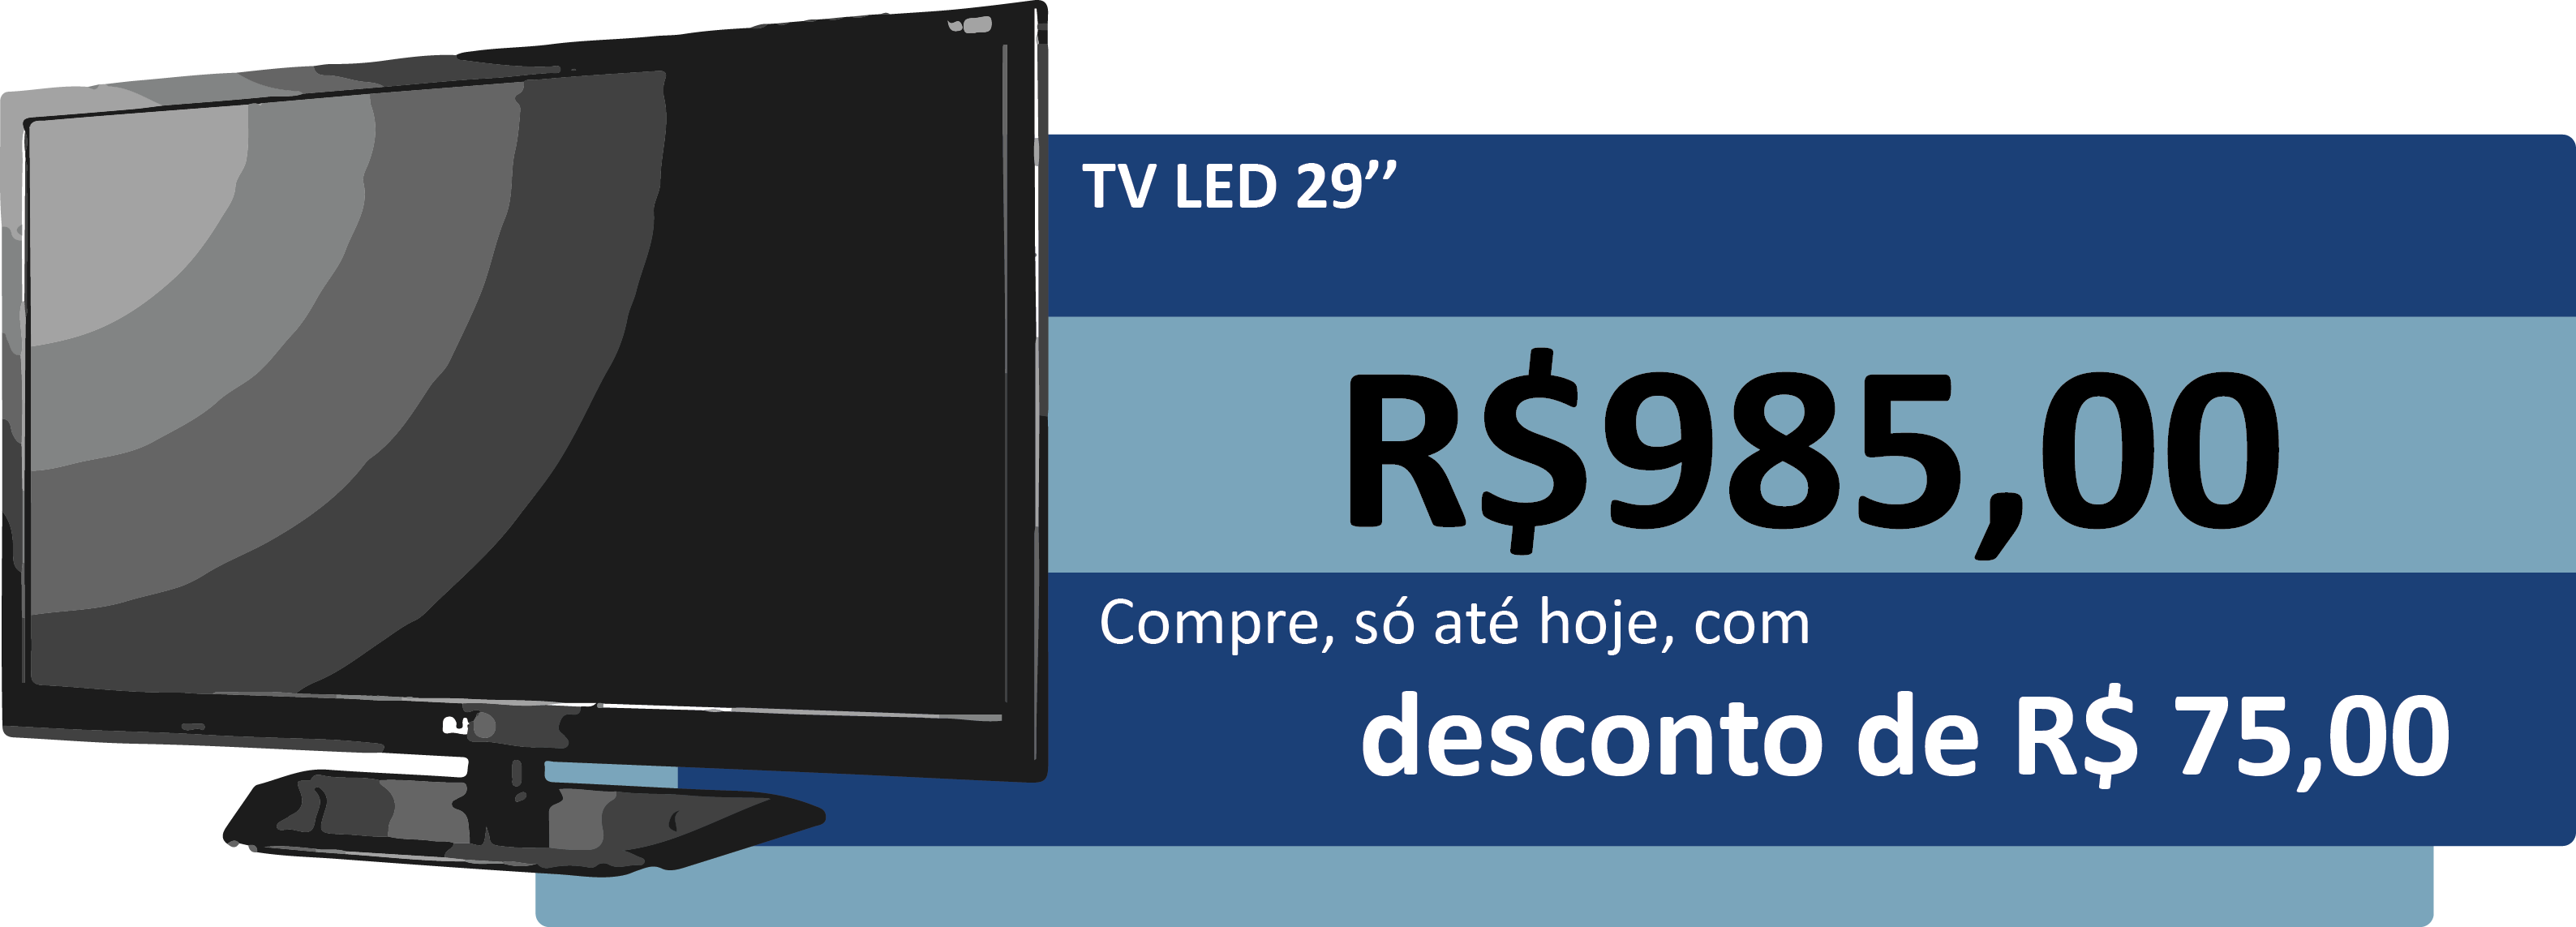
\includegraphics[width=.8\textwidth]{./media/image73.png}
\end{figure}

Uma pessoa que quiser aproveitar o desconto oferecido irá pagar nessa TV

\begin{escolha}
\item
  R\$ 985,00.
\item
  R\$ 75,00.
\item
  R\$ 910,00.
\item
  R\$ 1.060,00.
\end{escolha}

\num{2} Na lanchonete a que Augusto costuma ir com seus amigos, encontra-se a
seguinte tabela de preços:

\begin{longtable}[]{@{}ll@{}}
\toprule
\hline
\textbf{Produtos} & \textbf{Valor por unidade}\tabularnewline
\hline
\midrule
\endhead
Pão de queijo & R\$ 3,00\tabularnewline
\hline
Bombom & R\$ 5,00\tabularnewline
\hline
Suco & R\$ 6,00\tabularnewline
\hline
Doce & R\$ 4,50\tabularnewline
\hline
Refrigerante & R\$ 4,50\tabularnewline
\hline
Cachorro-quente & R\$ 12,00\tabularnewline
\bottomrule
\end{longtable}

Na última vez que Augusto foi a esse lugar, ele comprou 1 bombom, 2
sucos e 2 cachorros-quentes. Qual o valor gasto por Augusto nesse dia?

\begin{escolha}

\item
  R\$ 18,00.
\item
  R\$ 28,00.
\item
  R\$ 30,00.
\item
  R\$ 41,00.
\end{escolha}

\num{3} Júlia irá trocar suas notas por moedas para guardar tudo em seu
cofrinho. Ela quer trocar suas notas por moedas de 1 real.

Marque a
alternativa que traz o número correto de moedas de 1 real que ela
irá receber pelas suas notas quando efetuar a troca.

\begin{figure}[htpb!]
\centering
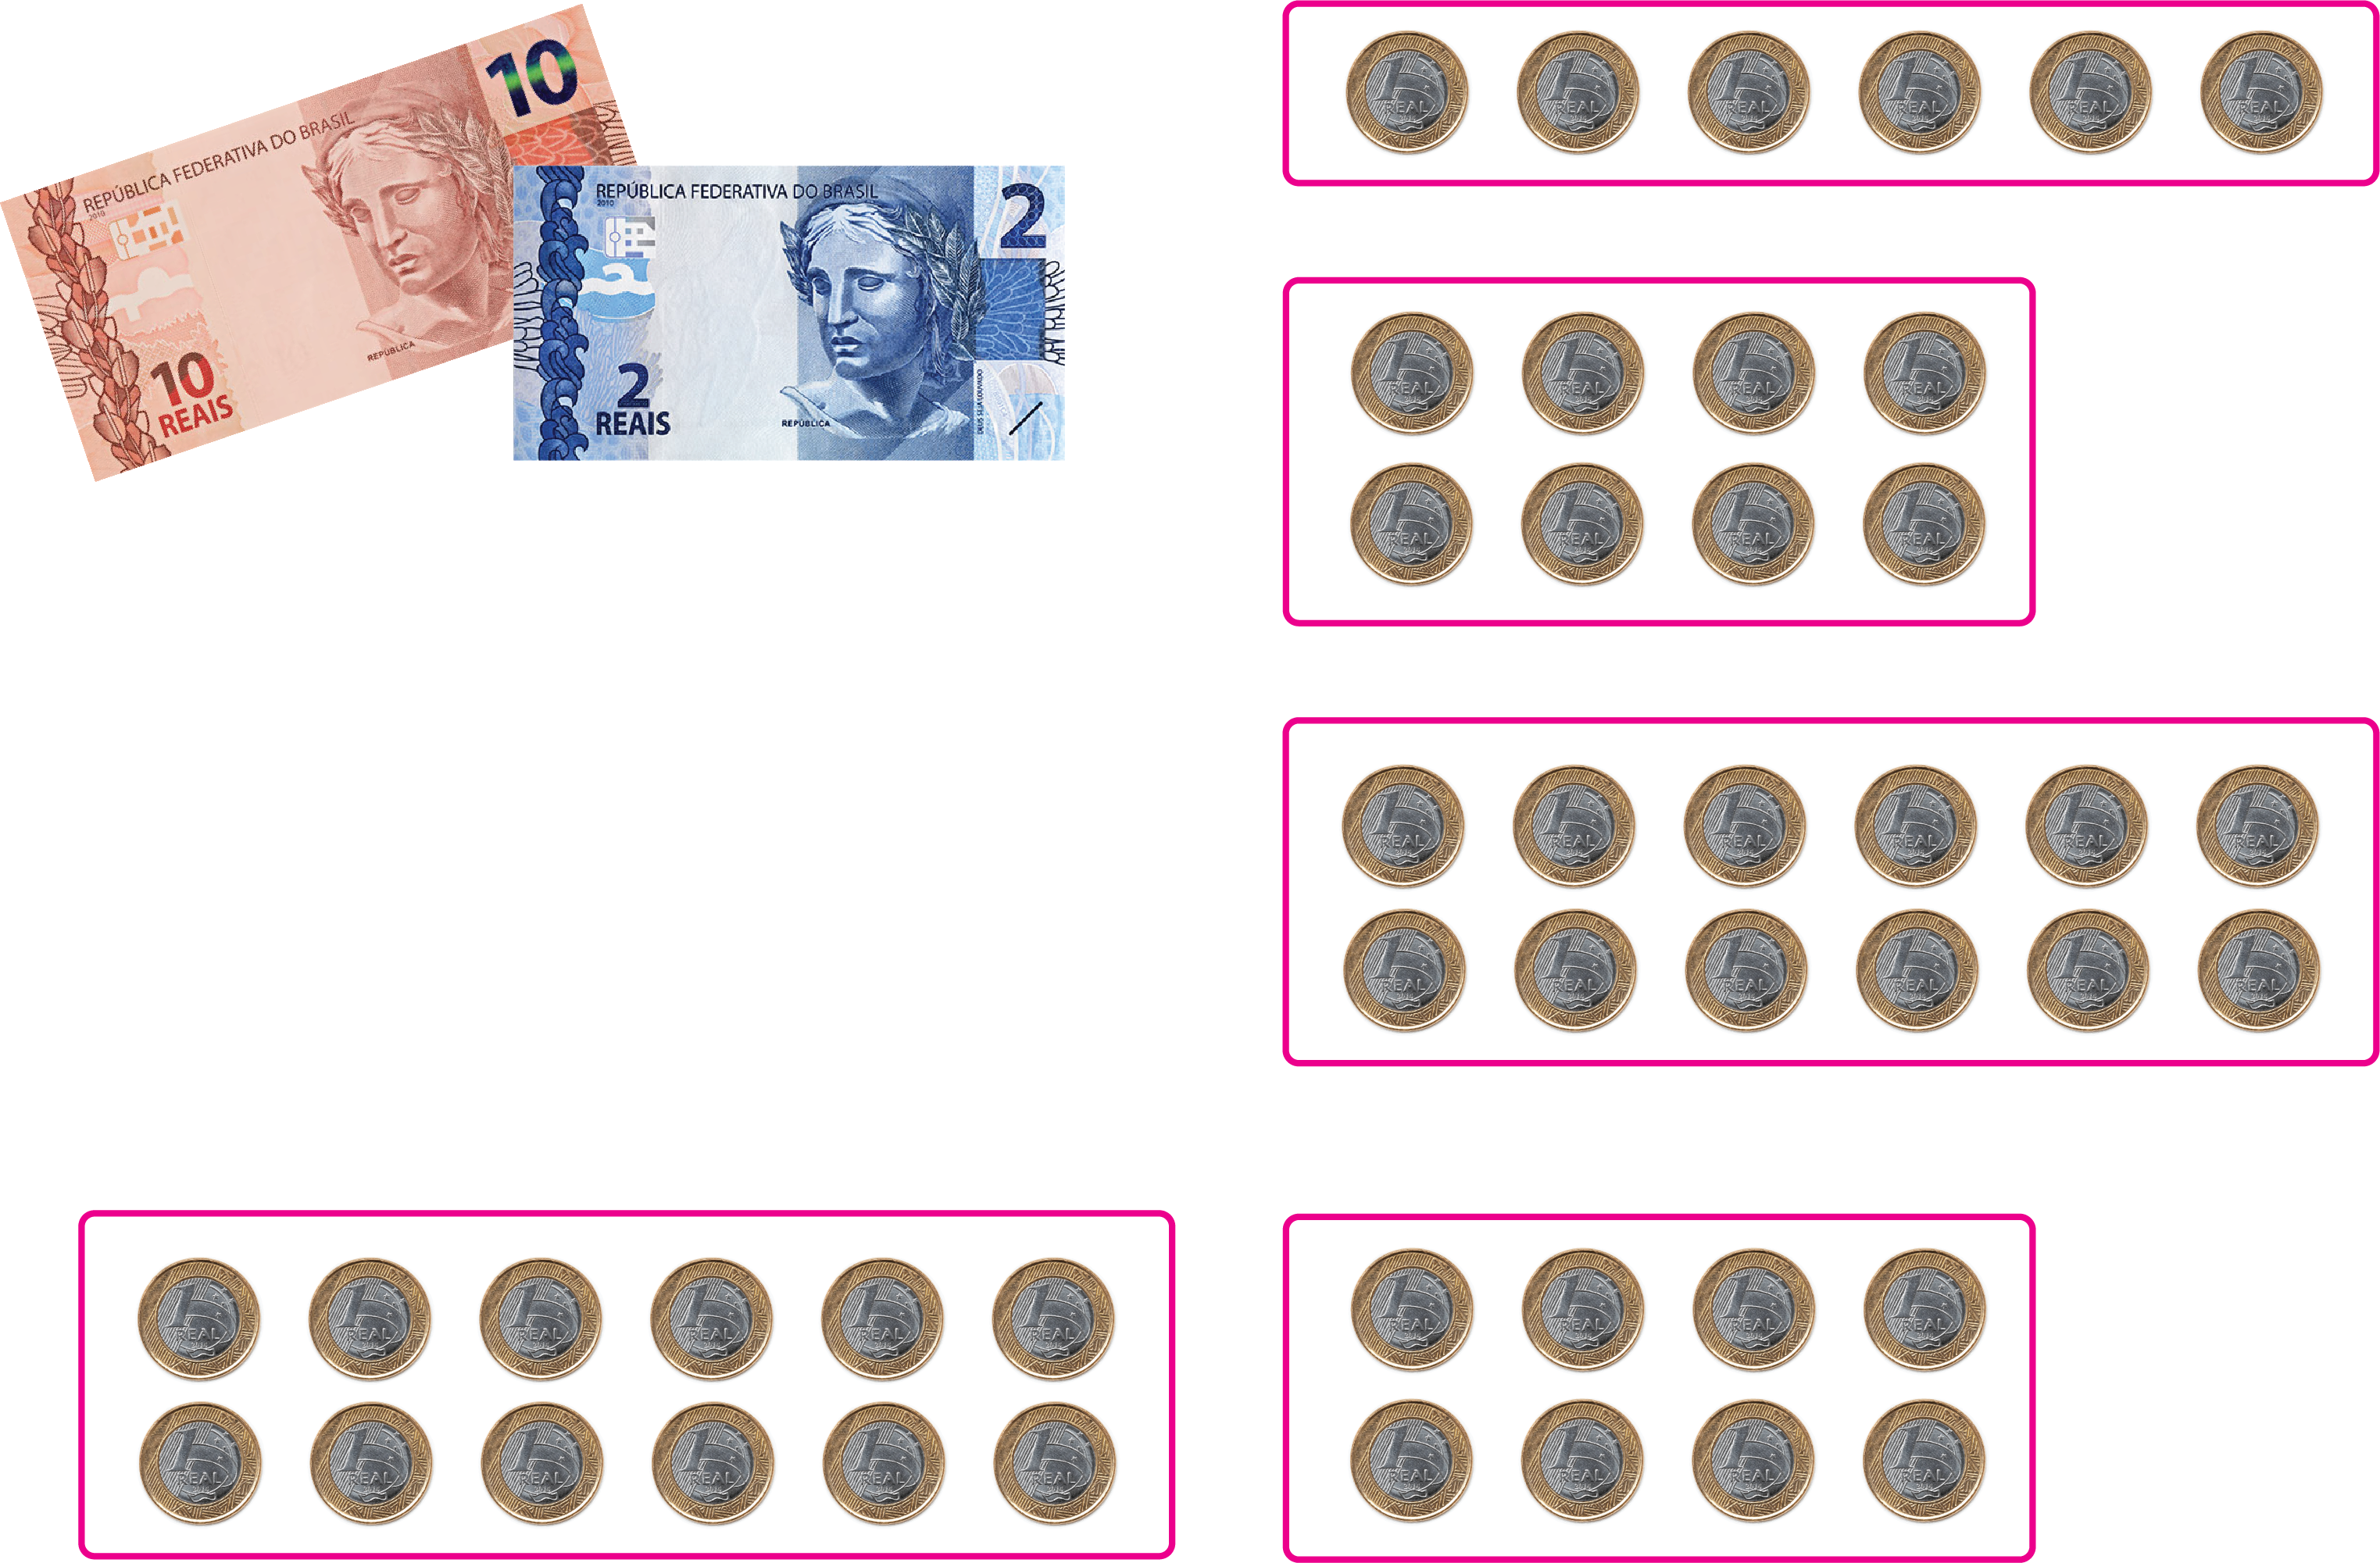
\includegraphics[width=\textwidth]{./media/image74.png}
\end{figure}

